\section{Bệnh án điện tử}
\begin{frame}{Bệnh án điện tử}
\putlogo
\begin{itemize}
	\item Là tài liệu ghi chép thông tin sức khỏe của bệnh nhân trong quá trình khám chữa bệnh
	\begin{itemize}
		\item Thông tin quản lý
		\item Dữ liệu lâm sàng và cận lâm sàng
	\end{itemize}
	\item Lợi ích từ bệnh án điện tử
	\begin{itemize}
		\item Thuận tiện lưu trữ
		\item Dễ dàng chia sẻ
	\end{itemize}
	\item Tồn tại dưới dạng tường thuật, không có cấu trúc
	\item Một hướng nghiên cứu được quan tâm: {\color{red} phân giải đồng tham chiếu}
\end{itemize}
\end{frame}

\section{Phân giải đồng tham chiếu}
\begin{frame}{Phân giải đồng tham chiếu}
\putlogo
\begin{itemize}
	\item Là xác định 2 hay nhiều khái niệm cùng chỉ một thực thể trong thế giới thực
\end{itemize}
\begin{figure}[ht!]
\centering
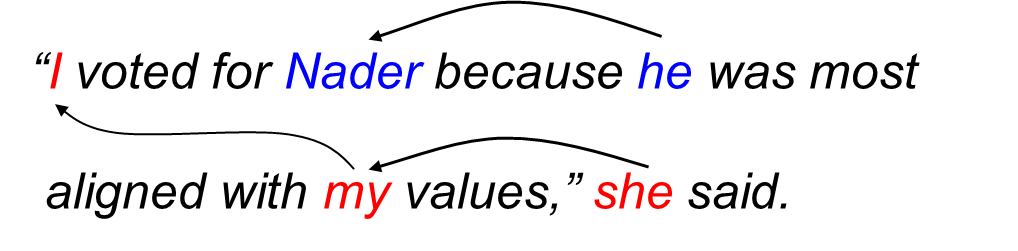
\includegraphics[width=0.5\textwidth]{./img/corefexample.png}
\end{figure}
\begin{itemize}
	\item Phụ thuộc vào ngữ cảnh
	\item Có 3 mô hình học máy được đề xuất:
	\begin{itemize}
		\item Cặp khái niệm
		\item Đề cập thực thể
		\item Xếp hạng
	\end{itemize}
\end{itemize}
\end{frame}